% "Compositing shaders in X3D" by Michalis Kamburelis,
% for TPCG 2011.
% If accepted, this will be Copyright 2011 by EUROGRAPHICS, details later.

%% Template stuff begins here ------------------------------------------------

\documentclass{egpubl}
\usepackage{EGUKTPCG11}
\WsSubmission
% TODO: \WsPaper for final?
\electronicVersion

% for including postscript figures
% mind: package option 'draft' will replace PS figure by a filname within a frame
\ifpdf \usepackage[pdftex]{graphicx} \pdfcompresslevel=9
\else \usepackage[dvips]{graphicx} \fi

\PrintedOrElectronic

% prepare for electronic version of your document
\usepackage{t1enc,dfadobe}

\usepackage{egweblnk}
\usepackage{cite}

%% Template stuff ends here ------------------------------------------------

% This is really the only sensible way to make breaking of monospace text
% (everything inside \texttt, including (but not limited) to urls).
% Otherwise, the monospace text flows outside of the column all over the place.
\sloppy

\usepackage{needspace}

%% Put float in a nice box,
%% http://en.wikibooks.org/wiki/LaTeX/Floats,_Figures_and_Captions
\usepackage{float}
\floatstyle{boxed}
\newfloat{mycodecore}{H}{listofmycode}
\floatname{mycodecore}{}

% Fix mycodecore: it has additional vertical line at the bottom after the frame.
% Possibly due to Verbatim inside?
\newenvironment{mycode}
{\begin{mycodecore}}
{\end{mycodecore}
\vspace{-0.1in}}

%% Use verbatim that allows \latex commands inside,
%% highly useful for my node spec figures.
%% See http://scott.sherrillmix.com/blog/category/programmer/latex/,
%% http://www.ctan.org/tex-archive/macros/latex/contrib/fancyvrb/
\usepackage{fancyvrb}

%% Without this, figure* can only go to the top (or separate page).
%% http://en.wikibooks.org/wiki/LaTeX/Floats,_Figures_and_Captions#Wide_figures_in_two_column_documents
\usepackage{stfloats}

%% Bold inside our code/spec samples.
\newcommand*{\codeem}[1]{\textbf{#1}}

\title{Compositing Shaders in X3D}

\author{1} % TODO: submission id
%\author[M. Kamburelis]{M. Kamburelis$^{1}$\\
%  $^1$Institute of Computer Science, University of Wroc{\l}aw, Poland}
%\author{(Author identification removed.)\thanks{e-mail: xxx@xxx.xxx}\\Xxx\\Xxx}

% For Web3D conf:
%\keywords{X3D, shaders, GLSL, effects, shadow maps, bump mapping}

\begin{document}

% TODO - restore?
%% \teaser{
%%   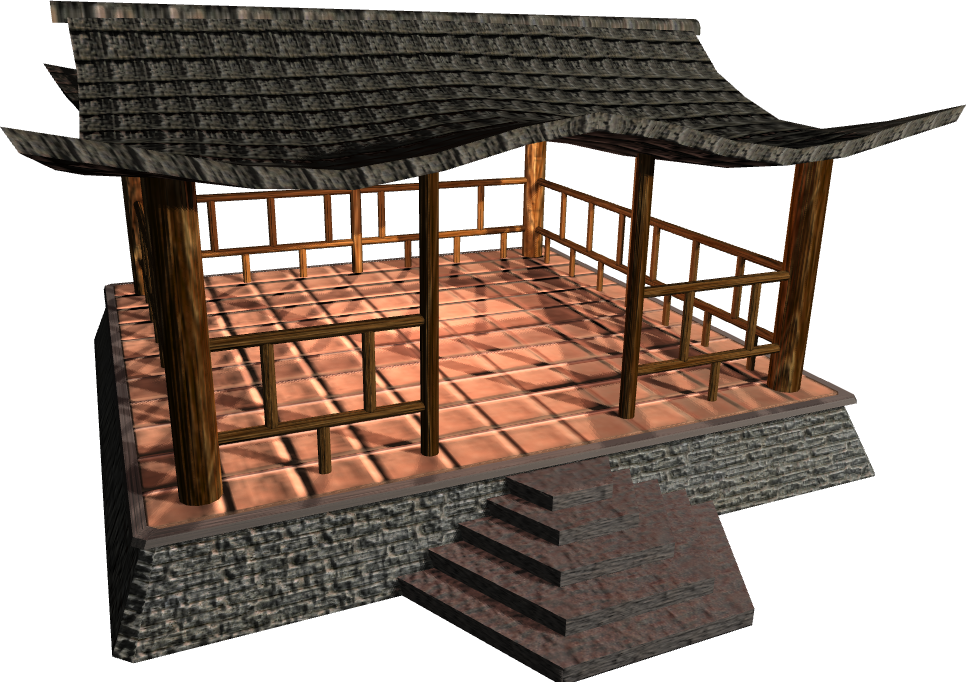
\includegraphics[width=2.19in]{rhan_shrine_5_everything}
%% %%  \caption{Bump mapping and 2 shadow maps on the same shape.}
%% }

\maketitle

\begin{abstract}
We present a new approach for implementing effects using the GPU shading languages.
Our effects seamlessly cooperate with each other and with
the shaders used internally by the 3D application.
Thus the effects are reusable, work in various combinations
and under all lighting and texture conditions.
%This makes the GPU shaders more usable for 3D content authors.
We have designed our effects to fit naturally in 3D scene graph formats,
in particular we present a number of extensions to the X3D standard.
Our extensions nicely integrate shader effects with X3D
%groups,
concepts like shapes, light sources and textures.

%% The browser implementation may also gain from using the same approach
%% for composing internal shaders.

\begin{classification}
  \CCScat{I.3.7}{Computer Graphics}{Three-Dimensional Graphics and Realism}{Color, shading, shadowing, and texture};
  \CCScat{I.3.6}{Computer Graphics}{Methodology and Techniques}{Languages, Standards}
\end{classification}

\end{abstract}

% For Web3D conf:
%\keywordlist

\section{Introduction}

% For Web3D conf:
%% The ``\copyrightspace'' command must be the first command after the
%% start of the first section of the body of your paper. It ensures the
%% copyright space is left at the bottom of the first column on the first
%% page of your paper.
%\copyrightspace

X3D \cite{x3d:spec} is an open standard for representing interactive 3D models,
with many advanced graphic features.

The X3D \textit{Programmable shaders component} \cite{x3d:shaders}
(part of the X3D standard) defines how \emph{shaders} can be assigned
to particular shapes. % and how they interact with other X3D features.
\emph{Shaders} are programs usually executed on the graphic processor unit
(GPU). They control the per-vertex and per-pixel processing,
for example summing the lights contribution
and mixing the texture colors. Since the authors, creators of 3D content,
can directly write and assign shaders to shapes, a myriad of interesting
graphic effects can be expressed in X3D models.

However, the shaders designed using the standard nodes
\textit{replace} the normal rendering functionality, not \textit{enhance} it.
This reflects the underlying API (like OpenGL or Direct 3D),
and the idea that shader code should be a complete and optimized program
designed for rendering a particular shape.

We argue that a different approach is needed in many situations.
Authors usually would like to keep the normal rendering features working,
and only add their own effects. The 3D renderer
implementation usually already has an extensive internal shaders system,
and the authors want to depend on these internal shaders
to do the common job.

As an example, consider this simplified lighting equation:
$$ \sum_{l\in Lights} shadow(l) * light\_color(l, material, normal(point)) $$
%% The \textit{shadow} function returns values in the [0..1] range,
%% scaling the light color. If the object is not in the shadow, it returns 1.
%% The \textit{normal} function returns a normal vector at given point.
Different effects want to change various parts of this equation,
without touching the others.
For example, the \textit{shadow} function may check a shadow map pixel,
or (when shadow map is not available) always return 1.
The \textit{normal} function may take the vector straight from
the geometry description, or calculate it using a texture value (classic bump mapping).
See figure \ref{fig_bump_mapping_shadows}.
The \textit{light\_color} function may be replaced to use different
lighting models.
% (Phong, Ward, Cook-Torrance and so on).
Sometimes it makes sense to change these functions
for all the light sources, and sometimes only a specific light source
should behave differently.
Our approach allows you to do everything mentioned above.
%% by inserting a piece
%% of custom shader code into a calculation of a particular function.
%on a particular object.

\begin{figure*}[t]
  \centering
  %% 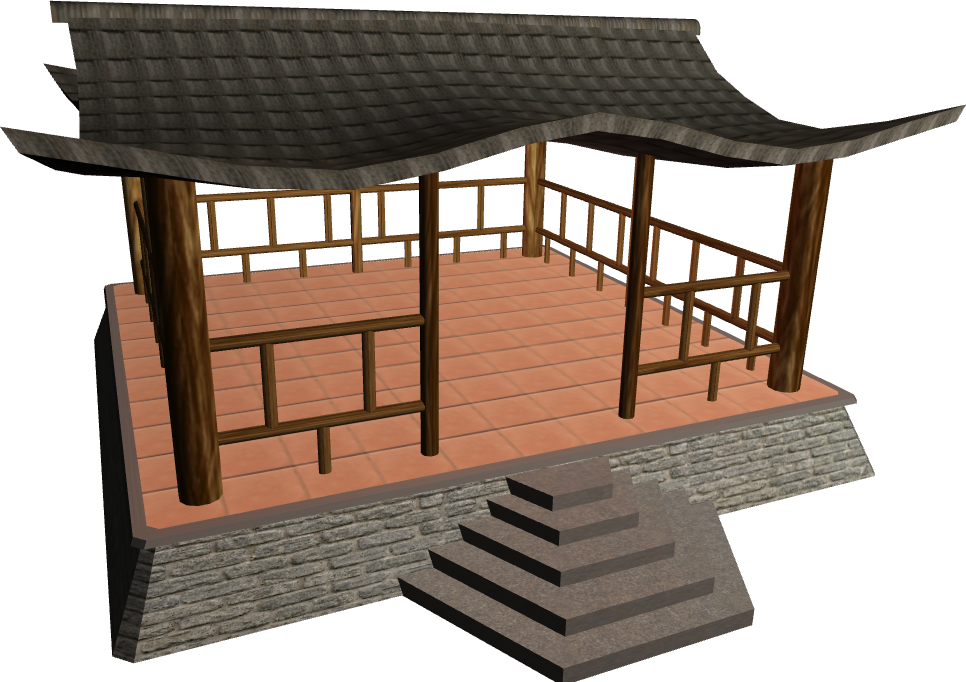
\includegraphics[width=2.0in]{rhan_shrine_0}
  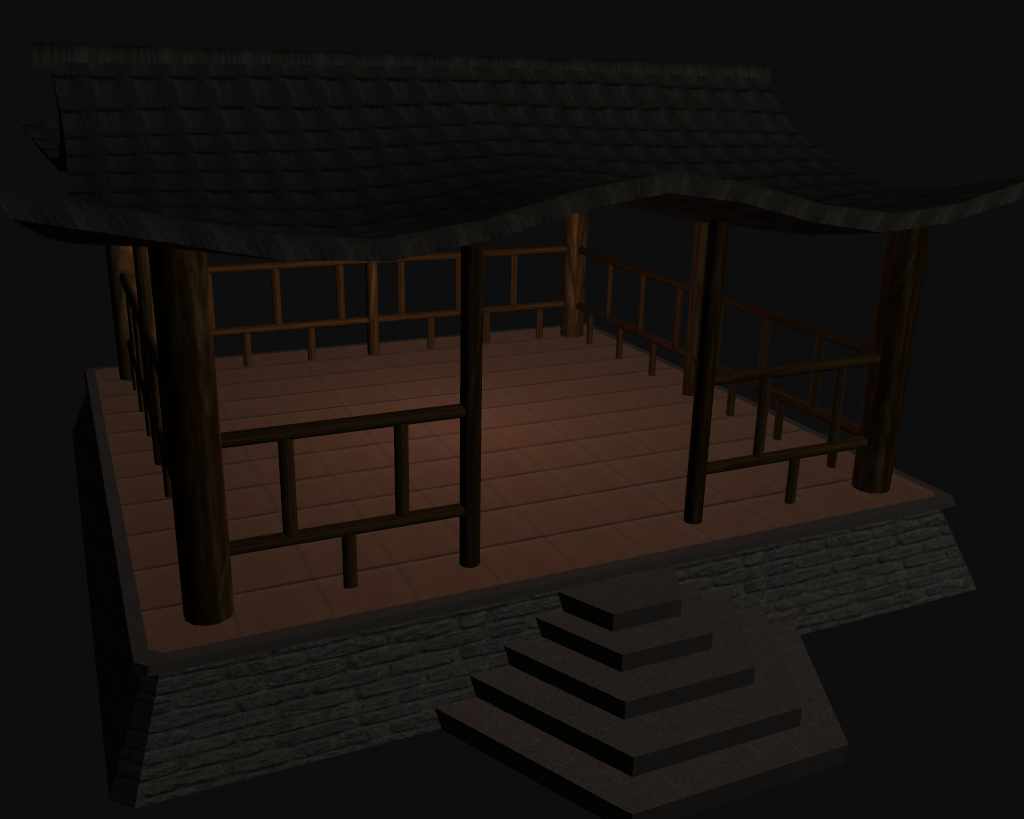
\includegraphics[width=2.0in]{rhan_shrine_1_per_pixel_lighting}
  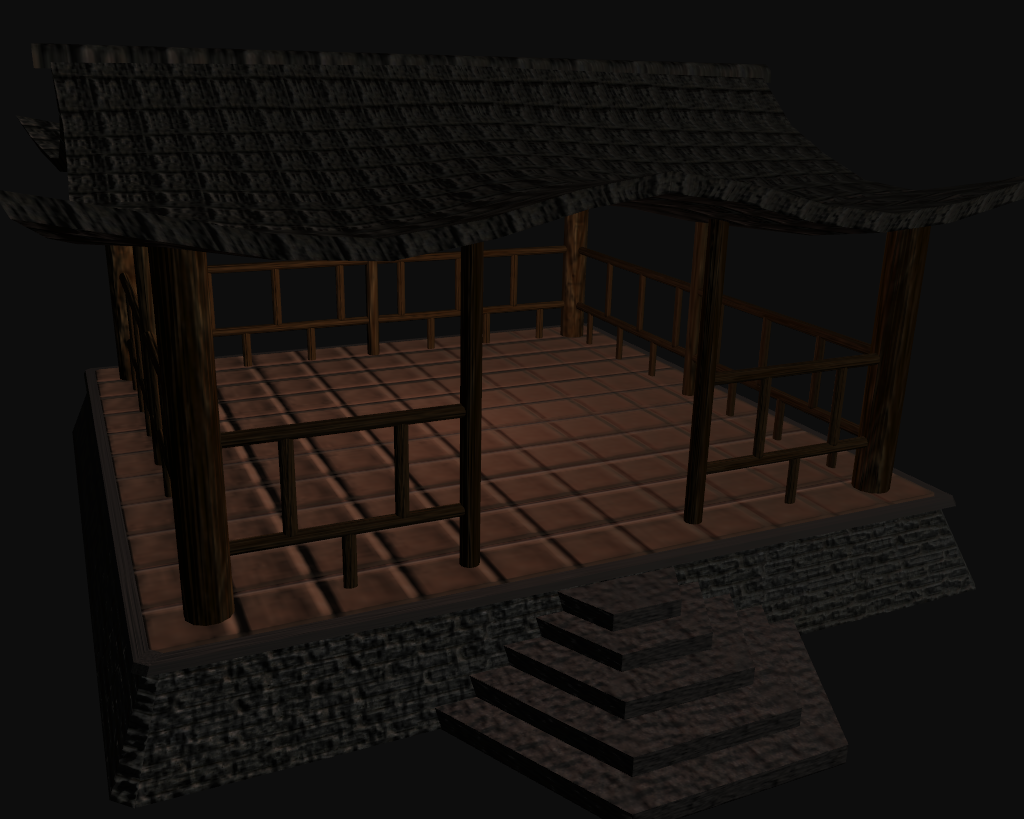
\includegraphics[width=2.0in]{rhan_shrine_2_bump_mapping}
  %% 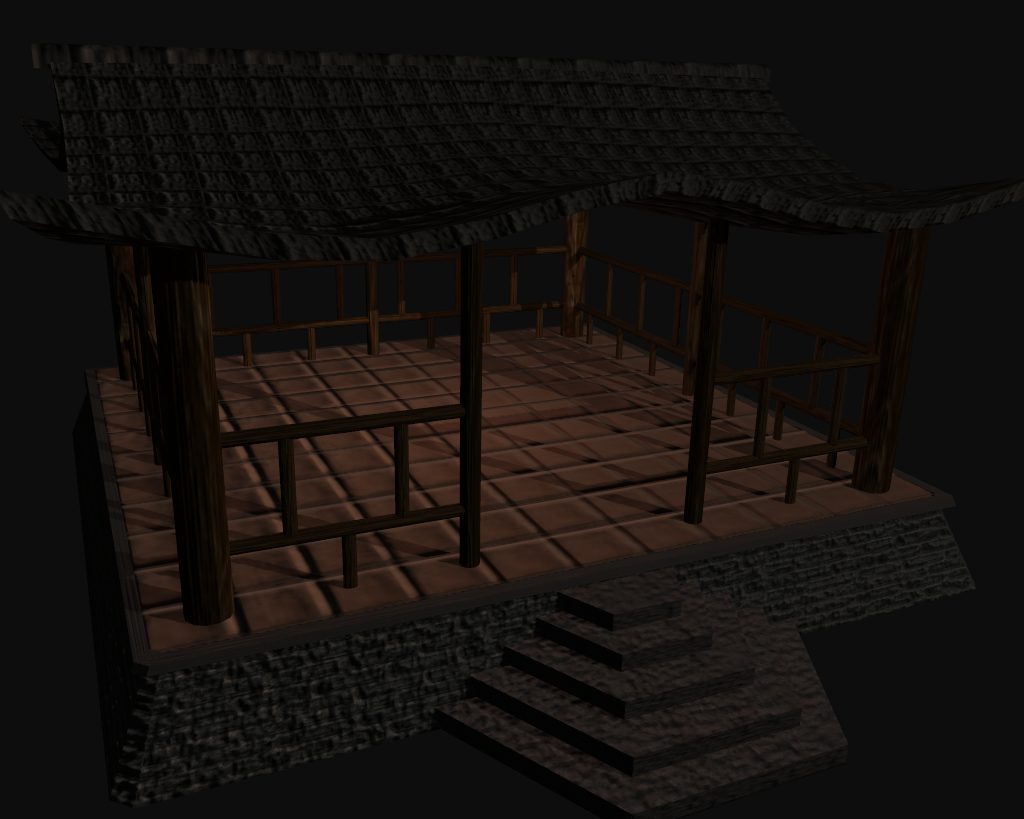
\includegraphics[width=2.0in]{rhan_shrine_3_shadow_1st}
  %% 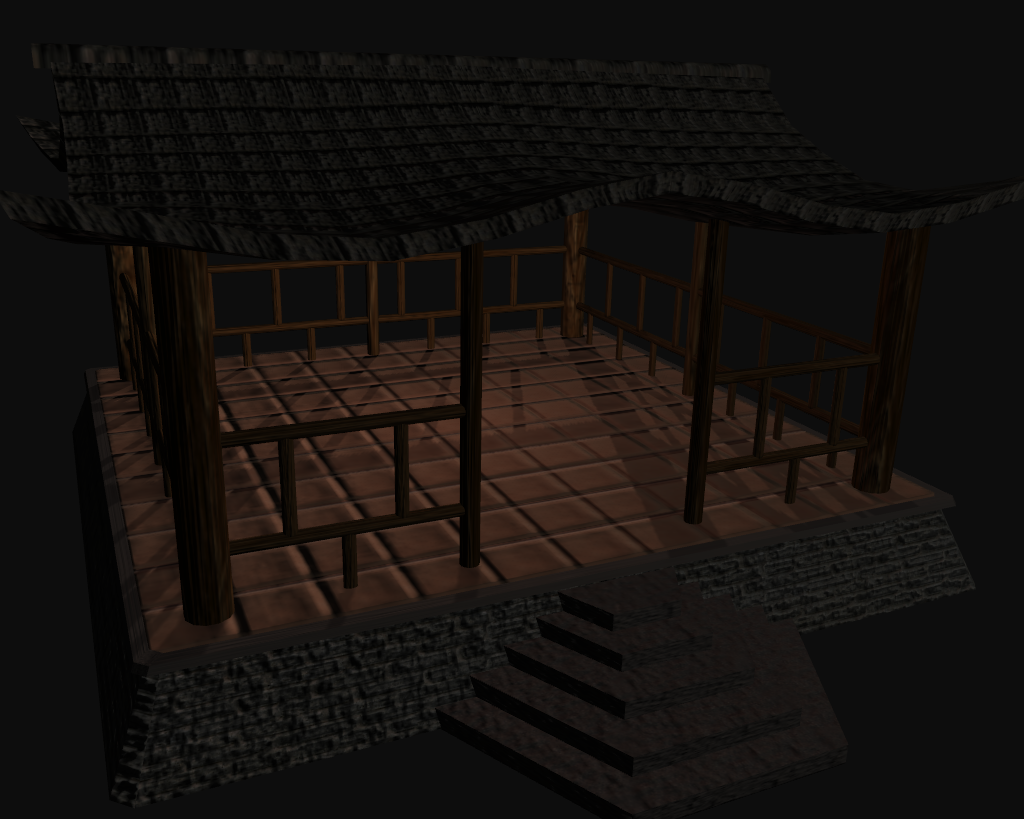
\includegraphics[width=2.0in]{rhan_shrine_4_shadow_2nd}
  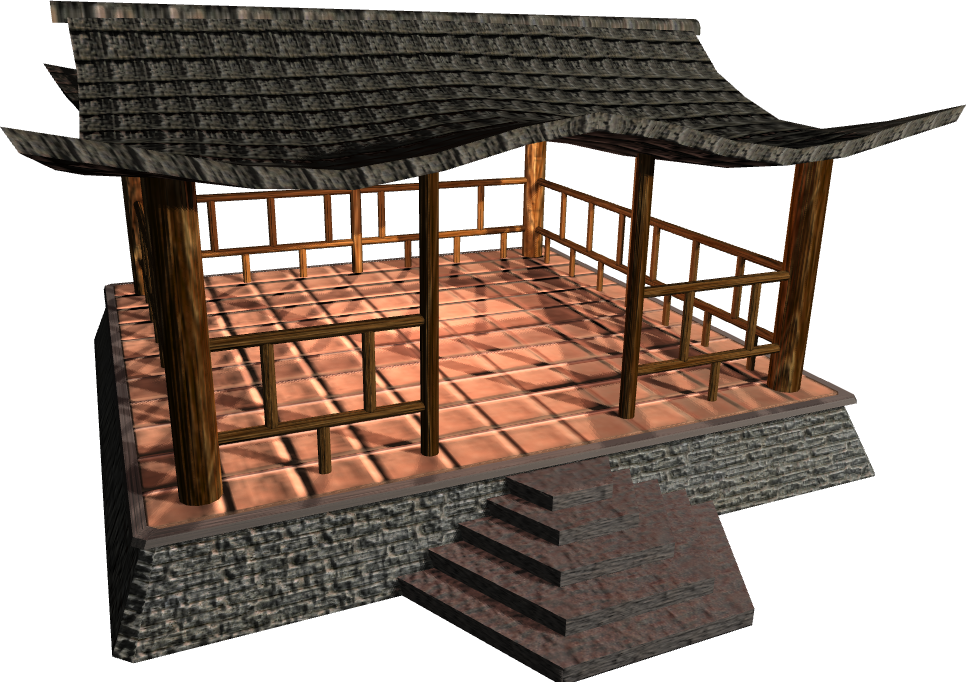
\includegraphics[width=2.0in]{rhan_shrine_5_everything}
  \caption{Japanese shrine model with more and more effects applied:
Phong shading (per-pixel lighting), bump mapping, shadows from two lights.
The model is based on \texttt{http://opengameart.org/content/shrine-shinto-japan}.}
  \label{fig_bump_mapping_shadows}
\end{figure*}

We present a system for creating effects by essentially compositing
pieces of a shader code. All the effects defined this way effortlessly
cooperate and can be combined with each other and with application internal
shaders. This makes shader programs:

\begin{enumerate}
\item Much easier to create. We can jump straight into the implementation
  of our imagined algorithm in the shader.
  We are only interested in modifying the relevant shader calculation
  parameter, and
  %don't need to care about the rest of the shader.
  we can completely ignore other parts of the shader.

\item Much more powerful. Our effect
  immediately cooperates with absolutely every normal feature of X3D rendering.
  This makes the implemented effect useful for a wide range of real uses,
  not only for a particular situation or a particular model (as it often happens
  with specialized shader code).
  All X3D light sources, textures, even other shader effects,
  are correctly applied.
\end{enumerate}

It is important that we still keep
the full power of a chosen GPU shading language.
We deliberately do not try to invent here a new language, or wrap existing
language in some cumbersome limitations.
%% This is most flexible for authors,
%% and it also allows an easy implementation --- there is no need for any complex
%% shading language processing inside the application.

\section{Motivation and previous work}

The popular real-time shading languages (OpenGL \texttt{GLSL} \cite{glsl:book}, NVidia \texttt{Cg}, Direct 3D \texttt{HLSL})
don't provide a ready solution for connecting shaders from independent sources.
The \texttt{CgFX} and HLSL \texttt{.fx} files encapsulate shading language code
in \emph{techniques} (for various graphic card capabilities),
and within a single technique specify operations for each rendering pass.
In neither case can we simply connect multiple shader source code files
and expect the result to be a valid program.

The X3D \textit{Programmable shaders component} \cite{x3d:shaders}
makes the three shading languages mentioned above available to X3D authors.
Complete shader code may be assigned to specific shapes.
Although it doesn't offer any way of compositing shader effects,
%the point of this component
%is to expose functionality that maps straightforward to graphic APIs like OpenGL.
this component is still an important base for our work. It defines
how to comfortably keep shader code inside X3D nodes, and how to pass uniform
values (including textures) to the shaders.

An oldest solution to combining effects, used even before the shading languages,
is a multi-pass rendering. Each rendering pass adds or multiplies
to the buffer contents, adding a layer with desired effect.
However, this is expensive --- in each pass we usually have to repeat
some work, at least transforming and clipping the geometry.
It is also not flexible --- we can only modify
the complete result of the previous pass.
%% In our work, we want to allow a single rendering pass to be as
%% powerful as it can.
Arranging shader functions in a pipeline has similar disadvantages
as multi-pass rendering, except there's no speed penalty in this case.

Common approach for writing a flexible shader code is to create
a library of functions, and allow the author to choose and compose them
in a final shader to achieve the desired look. But this approach is very limited,
as it doesn't allow to modify a particular calculation part without
replicating the algorithm outside of this calculation.
For example, if we want to scale the light contribution by a shadow function,
we will have to also replicate the code iterating over the light sources.

%% Another common solution is to arrange shaders in a pipeline, where one
%% shader processes the result of another. This can be visualized as
%% layers of materials, where each layer modifies the previous
%% color. It is actually similar to a multi-pass rendering approach,
%% except we don't lose speed on repeating the geometry transformation work.
%% Still it suffers from the same limitations, as we cannot change
%% the calculation within an existing layer, without replicating the whole
%% algorithm of this layer.

%% (see also http://groups.google.com/group/blendertorenderman/browse_thread/thread/aaf07831b91be9db?pli=1 , confirms my findings)

Sh (\URL{http://libsh.org/}, \cite{sh:book})
allows writing shaders code (that can run on GPU) directly inside a
C++ program.
%% For this, Sh extends the C++ language (through C++
%% operator overloading and macros tricks).
It allows an excellent
integration between C++ code and shaders, hiding the ugly details of
passing variables between normal code (that executes on CPU) and
shader code (that usually executes on GPU). We can use
object-oriented concepts to create a general shader that can
later be extended, for example by overriding virtual
methods. However, this is a solution closely coupled with C++. It's
suitable if we have a 3D engine in C++, and we want to use it in
our own C++ program and extend its shaders. Our solution is simpler,
treating shader effects as part of the 3D content, and can
be integrated into a renderer regardless of it's programming language.
Invoking a compiler to generate a
final GPU shader, not to mention forcing users to learn C++, is out of the
question.

OGRE (\URL{http://www.ogre3d.org/}), an open-source 3D engine written in C++, has a system
for adding shader extensions (see \cite{ogre:shader}). Its idea is similar
to our system (enhance the built-in shaders with our own effects),
however the whole job of combining a shader is done by operating
on particular shader by C++ code. The developer has to code
the logic deciding which shaders are extended, and most of the specification
about how the extension is called is done in the C++ code.
This has the nice advantage of being able to encapsulate some fixed-function
features as well, however the whole system must be carefully controlled by
the C++ code. In our approach, we allow the authors to write direct shading
language code quickly, and the integration is built inside appropriate X3D nodes.

AnySL \cite{anysl} is an approach to integrate renderer
shaders with user shaders. We strive to do something more (allow effortless
integration between various user shaders too), and simpler (without
introducing any new shading language).

%% \cite{web3d2010:declarativeshader} presents a declarative approach
%% to an advanced shader in X3D. However, it only allows a fixed set
%% of functionality, kind od ,,advanced and exhanced material''.
%% It doesn't expose any shader functionality to the authors.
%% It merely allows the authors to use some advanced algorithms that in practice
%% will be usually implemented by shaders inside the application.

At the end, we would like to mention a solution from a completely
different domain, that is surprisingly similar to ours in some ways.
Drupal (\URL{http://drupal.org/}),
an open-source CMS system written in PHP,
has a very nice system of modules. Each module
can extend the functionality of the base system (or other module)
by implementing a \textit{hook}, which is just a normal PHP function
with a special name and appropriate set of parameters. Modules can also define
their own hooks (for use by other modules) and invoke them when appropriate.
This creates a system where it's trivially easy to define a hook,
and to use a hook.
Many modules can implement the same hook and cooperate without any problems.
%% The whole hook system is defined completely in PHP, as it's a scripting
%% language, and we can query the list of loaded functions by name,
%% and call function by its name.
Drupal approach is quite similar to our
core idea of combining effects. Our effects are similar to
Drupal's modules, and our ,,plugging points'' are analogous to Drupal hooks.

%% Our effects can define functions with special names to enhance
%% the standard shader behavior, just like Drupal modules can define functions
%% to act on an event from another module.
%% We can also define new plugs, for other effects to use.
%% Of course we also have some special problems
%% (shading language is quite far from a scripting language,
%% so calling the plugs must be implemented by text replacements)
%% and some special opportunities (we can define effects at
%% the appropriate nodes of X3D, like textures and lights sources,
%% as we don't want to throw all the effects in one bag).

% OpenSceneGraph:
% http://www.openscenegraph.org/projects/osg/wiki/Support/Tutorials/ShadersParameters
% http://www.openscenegraph.org/projects/osg/wiki/Support/Tutorials/ShadersIntroduction
% http://mew.cx/osg_glsl_july2005.pdf
% I see no way to connect shaders?
%
% Irrlight --- also no way to connect shaders?
%
% Blender Game Engine: no way to connect shaders, Python code can
% set the final (complete) shader source only?
% http://download.blender.org/documentation/GE/Blender.htm
% http://www.blender.org/development/release-logs/blender-248/realtime-glsl-materials/
% See also source, inside source/gameengine/:
% ./Ketsji/BL_Shader.h
% ./Ketsji/BL_Shader.cpp
% ./Ketsji/BL_BlenderShader.h
% ./Ketsji/BL_BlenderShader.cpp

\section{Extending the shaders with plugs}

The core idea of our approach is that the base shader code defines
points where calls to user-defined functions may be inserted. We call
these places \textit{plugs}, as they act like sockets where logic
may be added. Each plug has a name, and a given set of parameters.
The effects can use special function names, starting with \texttt{PLUG\_}
and followed by the plug name. These declarations will be found,
and the renderer will insert appropriate calls to them from the base shader.

A trivial example of an effect that makes colors two times brighter
is below. This example is presented in the X3D classic (VRML) encoding.
We can add this inside any \texttt{Appearance} node in the X3D file:

\begin{Verbatim}[commandchars=\\\{\},frame=single,fontsize=\small]
effects Effect \{
  language "GLSL"
  parts EffectPart \{
    type "FRAGMENT"
    url "data:text/plain,
\textbf{    void PLUG_texture_apply(}
\textbf{      inout vec4 fragment_color,}
\textbf{      const in vec3 normal)}
\textbf{    \{}
\textbf{      fragment_color.rgb *= 2.0;}
\textbf{    \}}"
  \}
\}
\end{Verbatim}

This defines a GLSL function named \texttt{PLUG\_texture\_apply}
within an \texttt{EffectPart} node. The call to this function will
be automatically inserted at the \texttt{texture\_apply} plug point in
the renderer internal shader. This particular plug,
the \texttt{PLUG\_texture\_apply}, is called after the normal texture colors
are applied, but before the alpha test, and is a usual place to ,,just modify the pixel color''.
\texttt{fragment\_color} is an \texttt{inout} parameter, by modifying it
we modify the color that will be displayed on the screen.

We have a reference of all the plugging points available in our implementation
on \URL{http://vrmlengine.sourceforge.net/compositing_shaders.php}.
For each plugging point,
like this \texttt{PLUG\_texture\_apply}, we define a list of parameters
(they have to be declared exactly the same in an effect), and we define
when it is called.

\needspace{1in}
Many usage scenarios are possible:

\begin{enumerate}

\item The \texttt{Effect} nodes may refer to plug names
defined inside the application internal shaders. This is the most usual case.
It allows the authors to extend or override a particular shading parameter.

\item The \texttt{Effect} nodes may also use the plug names defined
in the previous \texttt{Effect} nodes on the same shape.
It is trivially easy (you just add a ,,magic'' comment) to define
plugging points in your own shader code, and this way your own effects
can be customized.

\item Inside the application implementation, the same approach can be used
to implement some internal effects.
We have reimplemented many internal effects of our engine,
like the fog, shadow maps (see \cite{vrmleng:shadowmaps})
and the bump mapping to use our ,,plugs'' approach.
This made their implementation very clean, short
and nicely separated from each other. It also proves that
the authors have the power to implement such effects easily by themselves.

%% without any traditional hassles. For example, bump mapping can be
%% achieved using standard \texttt{ComposedShader} as well,
%% but then you have to write all this ,,boilerplate'' code to also deal
%% with all the possible lighting and textures configurations.
%% Well, the application is still useful to calculate nice tangent vectors,
%% although an authoring program could generate GLSL attributes for them as well.

%% Same thing with shadow maps, they only plug to the \texttt{light\_scale}
%% calculation of appropriate light.

\end{enumerate}

Actually, there are even more possibilities.
We have been talking above about the ,,application internal shaders'',
but the truth is a little more flexible.
When you place a standard shader node
(like a \texttt{ComposedShader} node for GLSL shaders) on the
\texttt{Appearance.shaders} list,
then it replaces the internal application shaders.
If you define the same (or compatible) plugging points inside your shader,
then the application effects will be even added to your own
shader. And of course user effects are added to your shader too.
This way we have made even the standard X3D shader nodes much more flexible.
Note that if you don't define any plugs inside your \texttt{ComposedShader} node,
it continues to function as before --- no effects, from application or author,
will be added.

\subsection{Effect node}

We define new \texttt{Effect} node that holds information about
the source code and uniform values specific to a given effect.

\begin{mycode}
\underline{Effect : X3DChildNode}
\begin{Verbatim}[commandchars=\\\{\},fontsize=\small]
SFString [] \codeem{language} ""
  # Language like "GLSL", "CG", "HLSL".
  # This effect will be used
  # only when the base renderer shader
  # uses the same language.
SFBool [in,out] \codeem{enabled} TRUE
  # Easily turn on/off the effect.
MFNode [] \codeem{parts} [] # EffectPart
  # Source code of the effect.

# A number of uniform values may also
# be passed to the shader:
fieldType []       fieldName
fieldType [in]     fieldName
fieldType [out]    fieldName
fieldType [in,out] fieldName
\end{Verbatim}
\end{mycode}

%% , just like
%% # for ComposedShader node

% Comments for ,,enabled'':
%% # You could also remove/add the node
%% # from the scene, but often toggling
%% # this field is easier for scripts.

\needspace{1in}
The effect source code is split into a number of parts:

\begin{mycode}
\underline{EffectPart : X3DNode, X3DUrlObject}
\begin{Verbatim}[commandchars=\\\{\},fontsize=\small]
SFString [] \codeem{type} "VERTEX"
  # Like ShaderPart.type:
  # allowed values are
  # FRAGMENT | VERTEX | GEOMETRY.
MFString [] \codeem{url} []
  # The source code, like ShaderPart.url.
\end{Verbatim}
\end{mycode}

  %% # May come from an external file (url),
  %% # or inline (following "data:text/plain,").
  %% # In XML encoding, may also be inlined in CDATA.

Inside the effect part source code, the functions that enhance
standard shaders behavior are recognized by names starting with \texttt{PLUG\_}.
Of course you can also define and use other functions.
You can pass uniform variables to the effect,
and you can pass varying variables between the vertex and fragment
parts, just like with standard shader nodes.

In a single \texttt{EffectPart} node, you can define many \texttt{PLUG\_}
functions. However, your plug functions must be defined in the appropriate
effect type. For example, you cannot use the \texttt{texture\_apply} plug within
a \texttt{VERTEX} shader.
If your effect requires some processing per-vertex and some per-fragment,
you will probably use two \texttt{EffectPart} nodes, with appropriate types.
While this may seem like an arbitrary limitation,
this reflects how shader parts are declared in shading languages with
separate namespaces for vertex and fragment parts (like GLSL).
A single part may declare many variables and functions,
but it must be completely contained within a given shader type.

Note that it is completely reasonable to have an \texttt{EffectPart} node
with source code that doesn't define any \texttt{PLUG\_xxx} functions.
Such \texttt{EffectPart} node may be useful for defining shading language
utility functions, used by the other effect parts.

For shading languages that have separate compilation units
(like the \emph{OpenGL Shading Language}) the implementation may choose to place
each effect part in such separate unit. This forces the shader code to be
cleaner, as you cannot use undeclared functions and variables from other parts.
It also allows for cleaner error detection (parsing errors will be detected
inside the given unit).

At one point we tried the approach
to not look at any special function names in a shader code,
and instead define a plug name in the separate field of the \texttt{EffectPart}
node. However, the renderer may need to know the full declaration
of a plug function, to make a forward or external declaration of it.
One way to overcome this problem was to force repeating this declaration
in another field. Another way was to split shader code into much more
parts (for example, one part declares the uniform variables, one part declares
the plug function, one part defines the function body and so on).
Both approaches seemed uncomfortable and not natural for authors,
and they didn't really offer much simpler implementation, so we dropped this idea.
The current approach, to find the declarations of \texttt{PLUG\_xxx} functions
inside a complete shader code, is easy to implement, and results in clean
shader code of the effects. It also allows us to naturally use
the separate compilation units in case of GLSL.

\subsection{Effects for particular shapes}

There are various places where an \texttt{Effect} node may be used.
If it's specific to a given shape appearance, you can place it
on the \texttt{Appearance.effects} list:

\begin{mycode}
\underline{Appearance}
\begin{Verbatim}[commandchars=\\\{\},fontsize=\small]
MFNode [] \codeem{effects} [] # Effect
\end{Verbatim}
\end{mycode}

All the effects on this list (with suitable language) will be used.
%% Note that this is different
%% than the \texttt{Appearance.shaders}, which chooses only one shader.
%% For effects, we choose all of them.
This allows authors to define a library of independent shader effects,
and then trivially pick desired effects for each particular shape.
Simply placing two effects on the \texttt{Appearance.effects} list
makes them cooperate correctly.
%% . This also allows to
%% define a library of effects, that can be composited without any work
%% needed by user.

\begin{figure}[H]
  \centering
  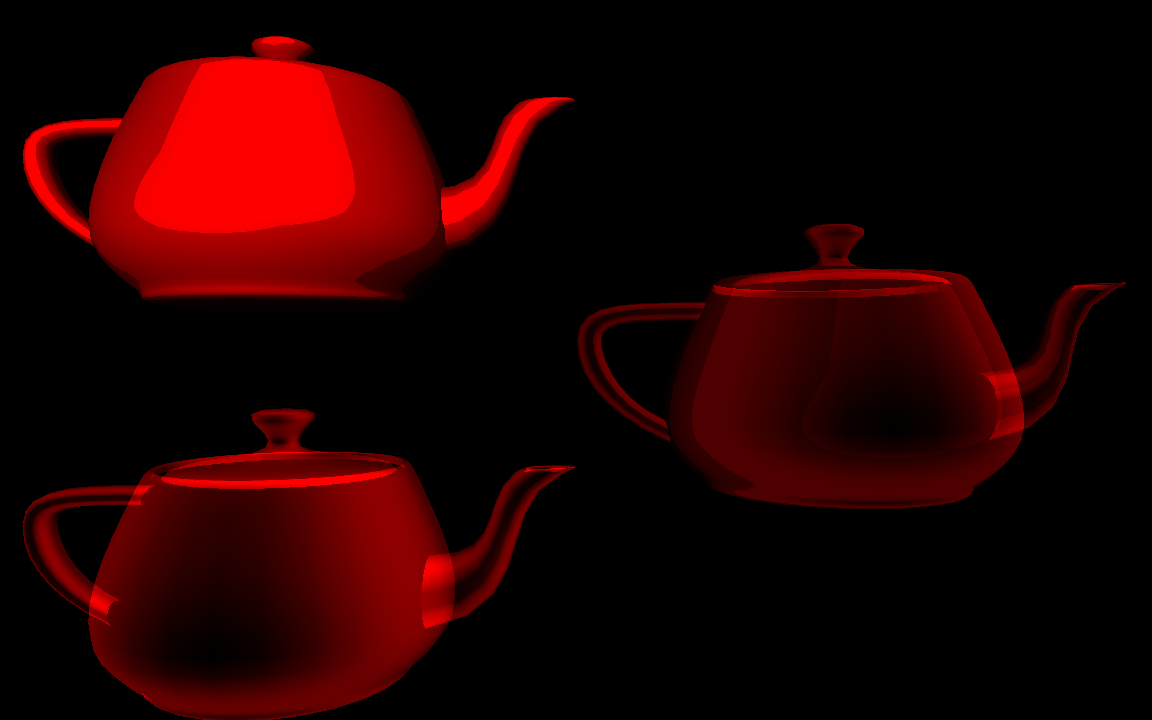
\includegraphics[width=3in]{fresnel_and_toon}
  \caption{Toon and Fresnel effects combined.}
\end{figure}

Note that all our nodes benefit from X3D mechanism to reuse the nodes
by reference (the \texttt{DEF} / \texttt{USE} keywords). Reusing the
\texttt{Effect} nodes
is most natural, and allows to combine existing effects in any desired way.
Reusing the \texttt{EffectPart} nodes is also useful, when some effects
would like to share a particular piece of code. For example,
you can create an \texttt{EffectPart} with a library of useful
shading language functions, and reuse if for various effects.

\begin{figure*}[t]
  \centering
  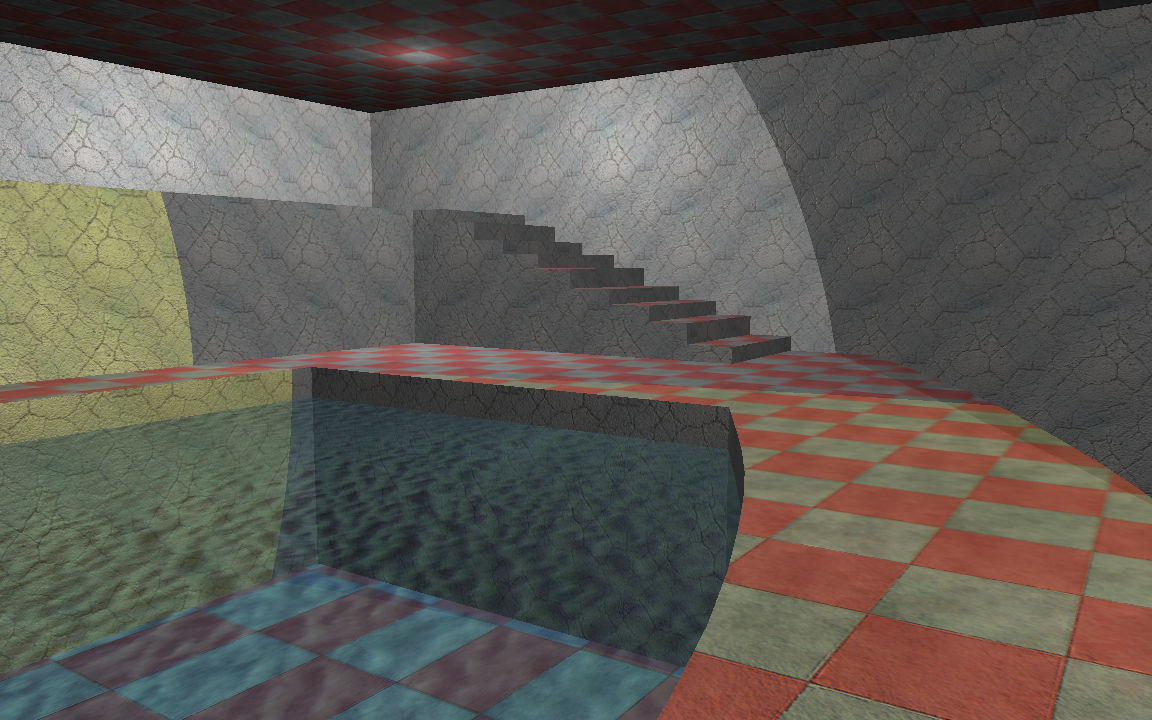
\includegraphics[width=2.0in]{volumetric_animated_fog_no_fog}
  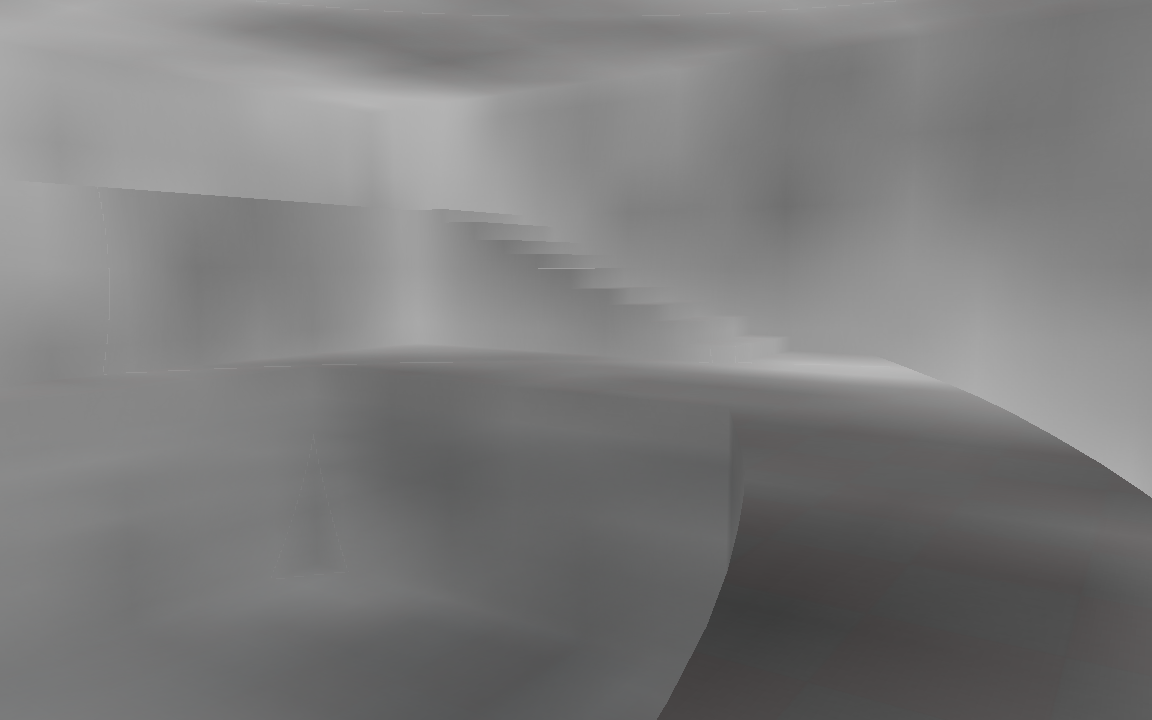
\includegraphics[width=2.0in]{volumetric_animated_fog_no_light}
  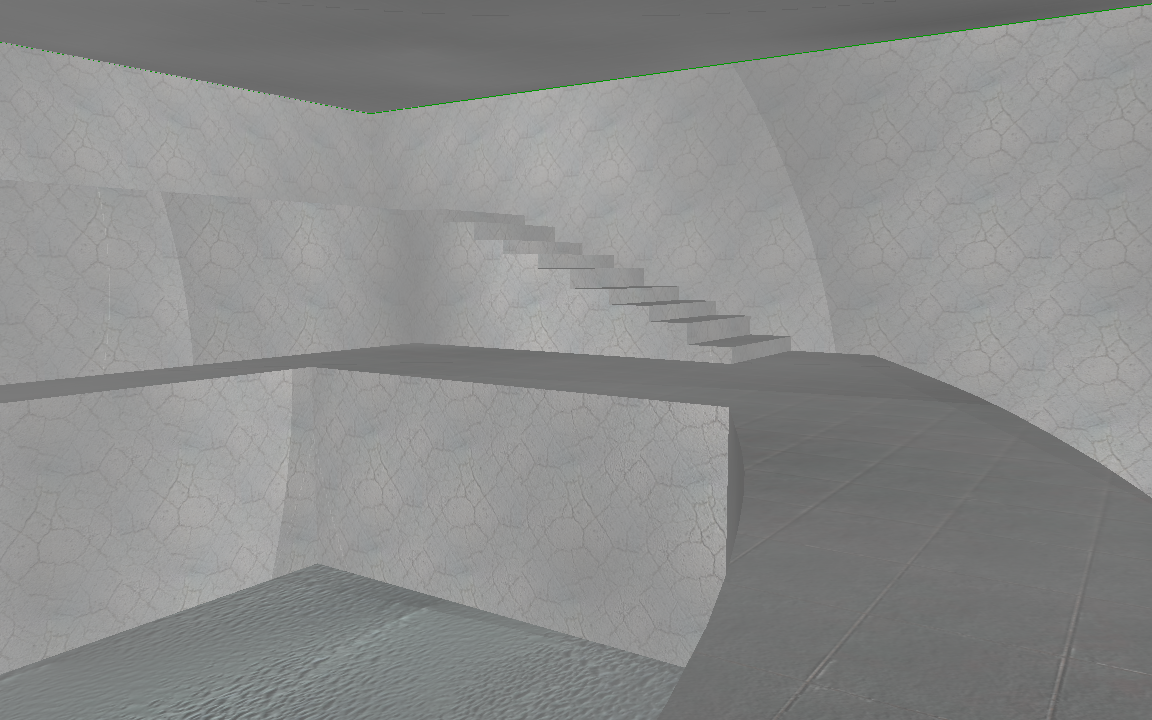
\includegraphics[width=2.0in]{volumetric_animated_fog_all}
  \caption{Volumetric fog scene: 1) No fog; 2) No lighting; 3) Lights and fog.
Note that the fog is assumed to have its own ambient lighting,
so it colors the image even in the 2) case.}
  \label{fig_fog}
\end{figure*}

\subsection{Effects for a group of nodes}

Our \texttt{Effect} node is a descendant of the abstract \texttt{X3DChildNode}.
As such it can be placed directly within X3D grouping nodes like
\texttt{Group}, \texttt{Transform} and at the top level of the X3D file.
Such effect will apply to all the shapes within the given group.
The scope rules follow the X3D conventions for other nodes,
like pointing device sensor nodes and \texttt{LocalFog}.

The \texttt{LocalFog} example is worth emphasizing. Using our system,
an X3D viewer can implement the \texttt{LocalFog} node as a prototype
that expands to our \texttt{Effect} node. This results in a 100\% correct
implementation of the standard \texttt{LocalFog} node, and is very easy.

As one of the demos, we have implemented a realistic
animated volumetric fog, where the fog density is stored in
a 3D smooth noise texture (idea from \cite{humus:volumetricfog}).
In a fragment shader, the 3D~texture is sampled
along the line between the camera and pixel position in the 3D~space. This makes a very
convincing effect of a dense fog. Since it is implemented as an effect,
it can be instantly used with various lighting and texturing conditions
--- it simply works for all X3D shapes. See figure \ref{fig_fog}.

\subsection{Light sources effects}

The nice feature of our system is that effects can be attached to various
types of objects, not just shapes. For example a particular light source
may have a shader effect assigned.
This allows to modify the contribution of a particular light.
For example the spot light shape can be modified, possibly
based on some texture information (see figure \ref{fig_fancy_spot}).
Or a different lighting model may be implemented, like anisotropic Ward
or Cook-Torrance.
To make this possible, we add the \texttt{effects} field to every light node:

\begin{mycode}
\underline{X3DLightNode}
\begin{Verbatim}[commandchars=\\\{\},fontsize=\small]
MFNode [] \codeem{effects} [] # Effect
\end{Verbatim}
\end{mycode}

\begin{figure}[H]
  \centering
  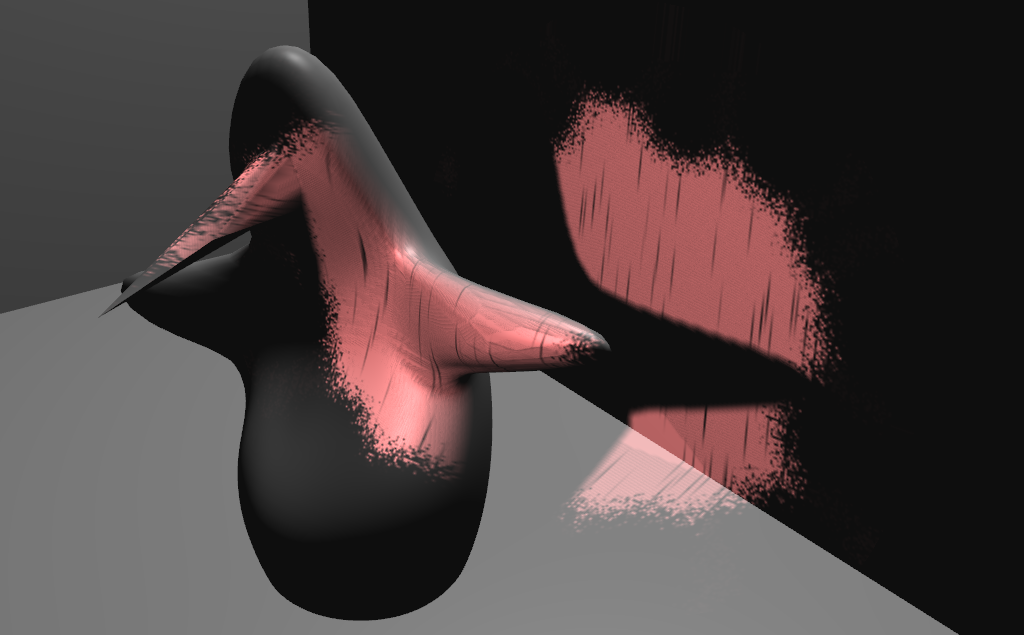
\includegraphics[width=2.5in]{fancy_light_spot_shape-cropped}
  \caption{Textured spot light with shadow.}
  \label{fig_fancy_spot}
\end{figure}

%% , or even replace the default
%% calculation of the light source contribution. In the second case,
%% the default calculation will not even be used in the shader,
%% so it will not slow down the calculation without a reason.

\subsection{Texture effects}

Just like the light sources, also each texture node may define its own effects:

\begin{mycode}
\underline{X3DTextureNode}
\begin{Verbatim}[commandchars=\\\{\},fontsize=\small]
MFNode [] \codeem{effects} [] # Effect
\end{Verbatim}
\end{mycode}

You can use the \texttt{effects} field
inside any \texttt{X3DTextureNode} to enhance and modify the look of any
standard texture node, like \texttt{ImageTexture}.
You can use a plug \texttt{texture\_color} to change the texture color,
knowing the current texture coordinates and other information.

\subsubsection{ShaderTexture effects}

We introduce a new X3D node designed specifically for generating
textures using the shaders. This is suitable
if your texture is defined completely using the shading language.
The texture contents are not stored anywhere (not even on GPU),
and the application doesn't manage any texture resources.
From a GPU point of view, there is no texture.
%\footnote{But the spoon is real,
%we swear.}.
There is only a shader function that generates colors
based on some vectors. By wrapping such function inside
the new \texttt{ShaderTexture} node, you can treat it much like other X3D textures.
In particular, you can provide texture coordinates (explicit or generated)
for the texture.
Effectively, it behaves like a normal texture node, with all the related
X3D features.

%% The new texture node specification:

\begin{mycode}
\underline{ShaderTexture : X3DTextureNode}
\begin{Verbatim}[commandchars=\\\{\},fontsize=\small]
MFNode [] \codeem{effects} [] # Effect
SFString [] \codeem{defaultTexCoord} "BOUNDS2D"
  # ["BOUNDS2D"|"BOUNDS3D"]
\end{Verbatim}
\end{mycode}

%% Actually, the \texttt{effects} field is already defined at
%% the \texttt{X3DTextureNode} class (see above). We just mention it here
%% for completeness.

You should include an effect overriding at least the \texttt{texture\_color}
plug, otherwise texture contents are undefined. Our implementation actually
sets the default texture color to pink (RGB(1,~0,~1)), so it stands out,
reminding you to override it.

The texture coordinates, or the algorithm to generate them,
can be explicitly specified, just like for any other texture in X3D.
%% . This follows the usual rules for all
%% when you place a \texttt{X3DTextureCoordinateNode} node
%% inside the geometry \texttt{texCoord} field.
%% Both explicit texture coordinate lists (\texttt{TextureCoordinate}
%% \texttt{TextureCoordinate3D}, \texttt{TextureCoordinate4D})
%% and the coordinate generator nodes
%% (like \texttt{TextureCoordinateGenerator}) are suitable.
%% %% , \texttt{ProjectedTextureCoordinate}
%% Note that our engine has some extensions to allow
%% the \texttt{"BOUNDS2D"} and \texttt{"BOUNDS3D"} values to be also
%% used for the \texttt{TextureCoordinateGenerator.mode} field, see
%% \cite{vrmleng:texcoordbounds}.
When the texture coordinates are not explicitly given,
the \texttt{defaultTexCoord} field determines how they are generated.
\texttt{"BOUNDS2D"} generates 2D texture coordinates,
adapting to the two largest bounding box sizes
(the 3rd texture coordinate is always 0). This is most comfortable
when the texture color depends only on the XY components of the texture coordinate.
The precise behavior
of \texttt{"BOUNDS2D"} follows the X3D \texttt{IndexedFaceSet} specification,
and the precise behavior of \texttt{"BOUNDS3D"} is described in
the \textit{Texturing3D} component of the X3D specification.

%%  (section \textit{"Texture coordinate generation for primitive objects"})
%%   is used.
%%   This adapts 3D texture coordinates to the bounding box sizes.
%%   It's most suitable for 3D textures (you can ignore the 4th texture coordinate
%%   component, or treat it as homogeneous, as \texttt{"BOUNDS3D"} will always
%%   set it to 1).

%% \end{enumerate}

%% The idea is that using a \texttt{ShaderTexture} should be as comfortable
%% as any other texture node.

%% Projective texture mapping by \texttt{ProjectedTextureCoordinate}
%% is also our extension, see \cite{vrmleng:projectivetexturing}.

\subsubsection{When to use the ShaderTexture}

For textures other than the \texttt{ShaderTexture},
when the \texttt{texture\_color} plugs are called,
the internal shaders have already calculated the initial texture
color by actually sampling the texture image. This is useful if you
want to modify this color. If you'd rather ignore the normal
sampled color, and always override it with your own, consider using
the special \texttt{ShaderTexture} node instead. Using
a normal texture node (like \texttt{ImageTexture}) for this
would be uncomfortable, as you would have to load a dummy texture image,
and the shaders could (depending on optimization) waste some time
on calculating a color that will be actually ignored later.

Note that in all cases (effects at \texttt{ImageTexture},
at \texttt{ShaderTexture}, etc.) you can always use additional
textures inside the effect. Just like inside a standard \texttt{ComposedShader},
you can declare an \texttt{SFNode} field inside an \texttt{Effect}
to pass any texture node to the shader as a uniform value.
This allows to combine any number of textures inside an effect.
The only difference
between \texttt{ShaderTexture} and other textures is what the system
does automatically for you, that is what color is passed
to the first \texttt{texture\_color} plug.

\begin{figure}[H]
  \centering
  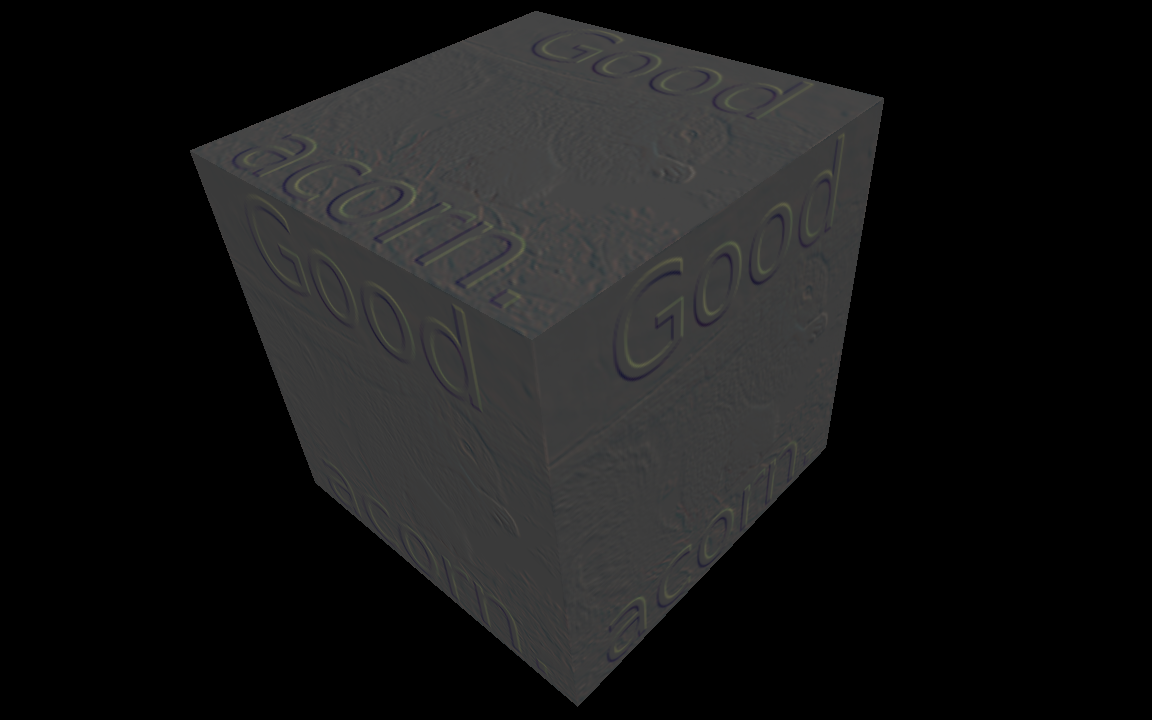
\includegraphics[width=3in]{shader_texture_edge_detection}
  \caption{ShaderTexture doing an edge detection operation on a normal ImageTexture.}
\end{figure}

%% \subsubsection{Independence from texture filtering}

%% Note that the shader effects for textures are calculated at each screen fragment
%% (not at each texel). So your effects are not concerned about the texture size
%% or texture filtering options. You just use the interpolated texture
%% coordinates in the \texttt{texture\_color} plug.

%% \begin{figure}[H]
%%   \centering
%%   
\includegraphics[width=3in]{shader_texture_no_filtering_problems-cropped}
%%   \caption{Yellowish arc is done by a texture effect, and so is not
%%     affected by the pixelated look of the base image texture.}
%% \end{figure}

\setcounter{figure}{7}
\begin{figure*}[b]
  \centering
%  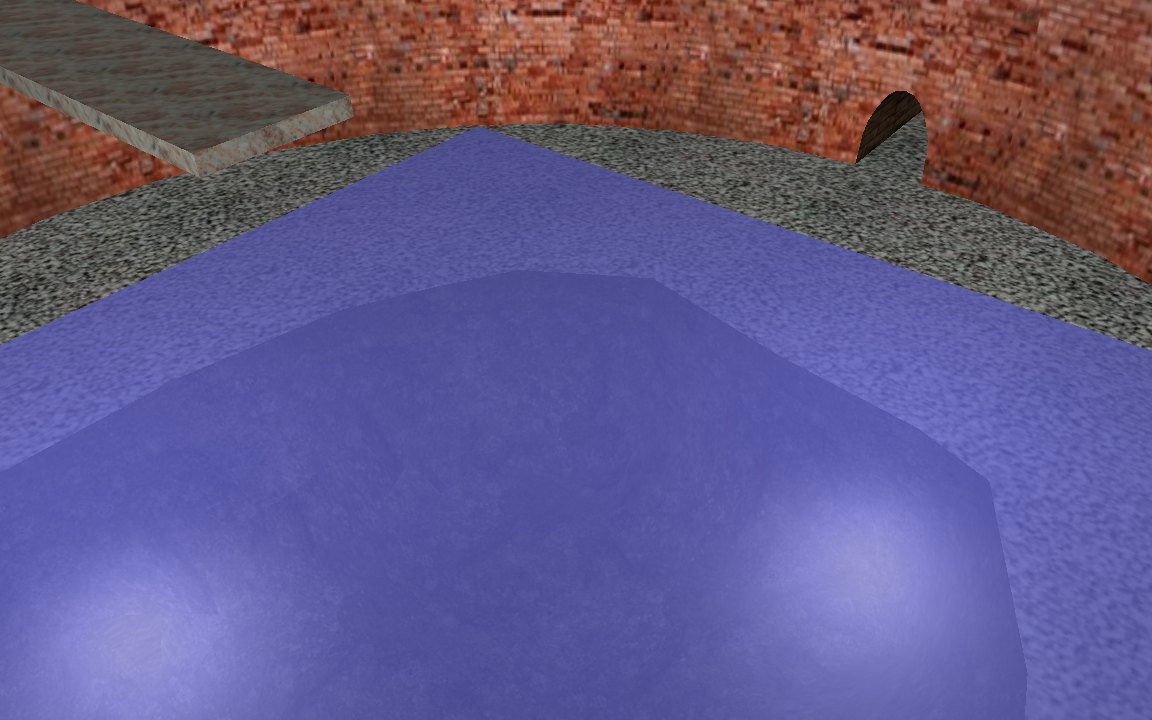
\includegraphics[width=2.3in]{water_shaders_0}
  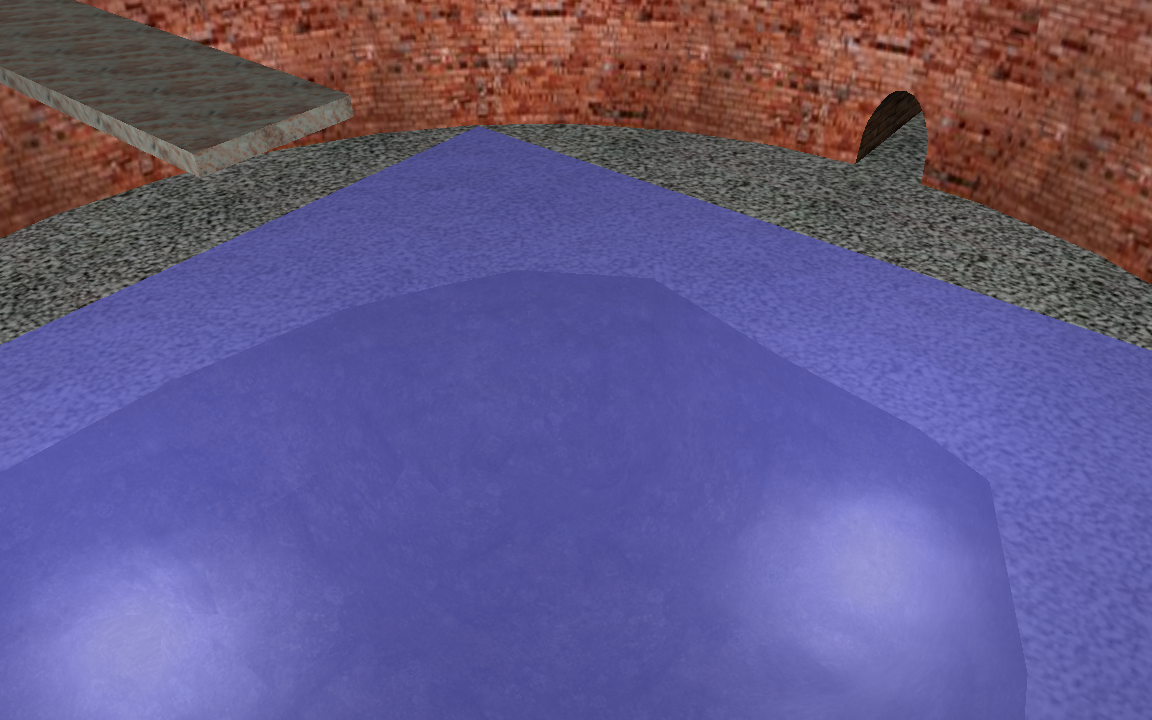
\includegraphics[width=2.0in]{water_shaders_1}
  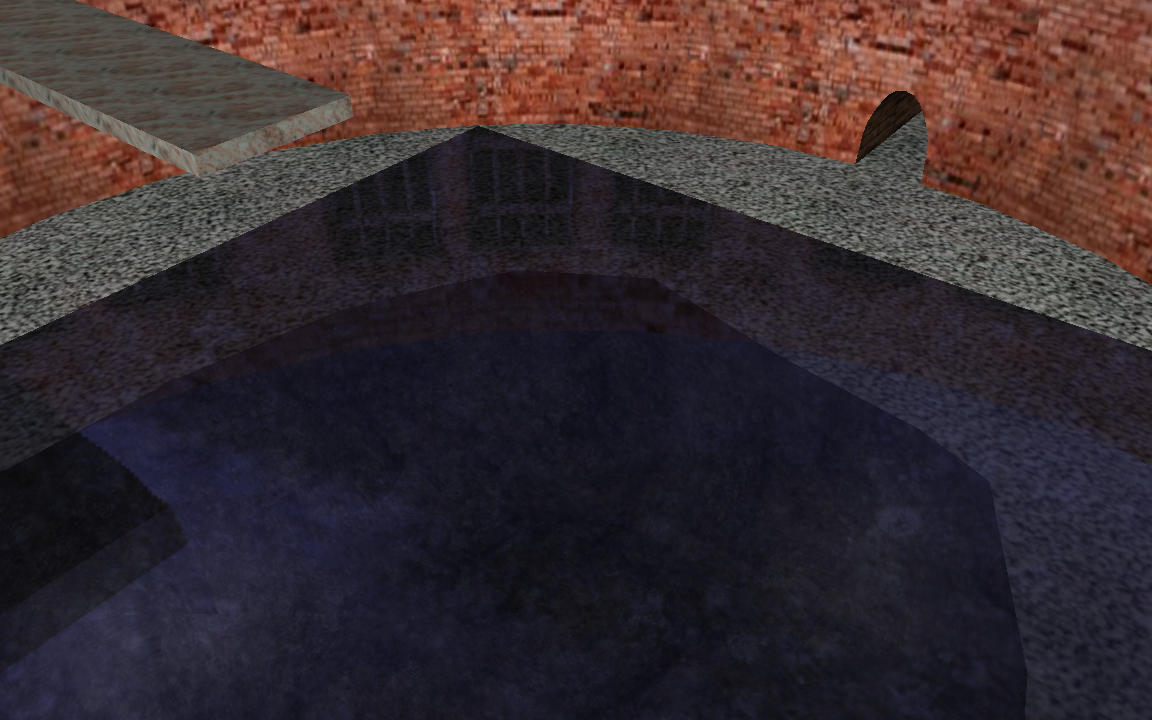
\includegraphics[width=2.0in]{water_shaders_2}
  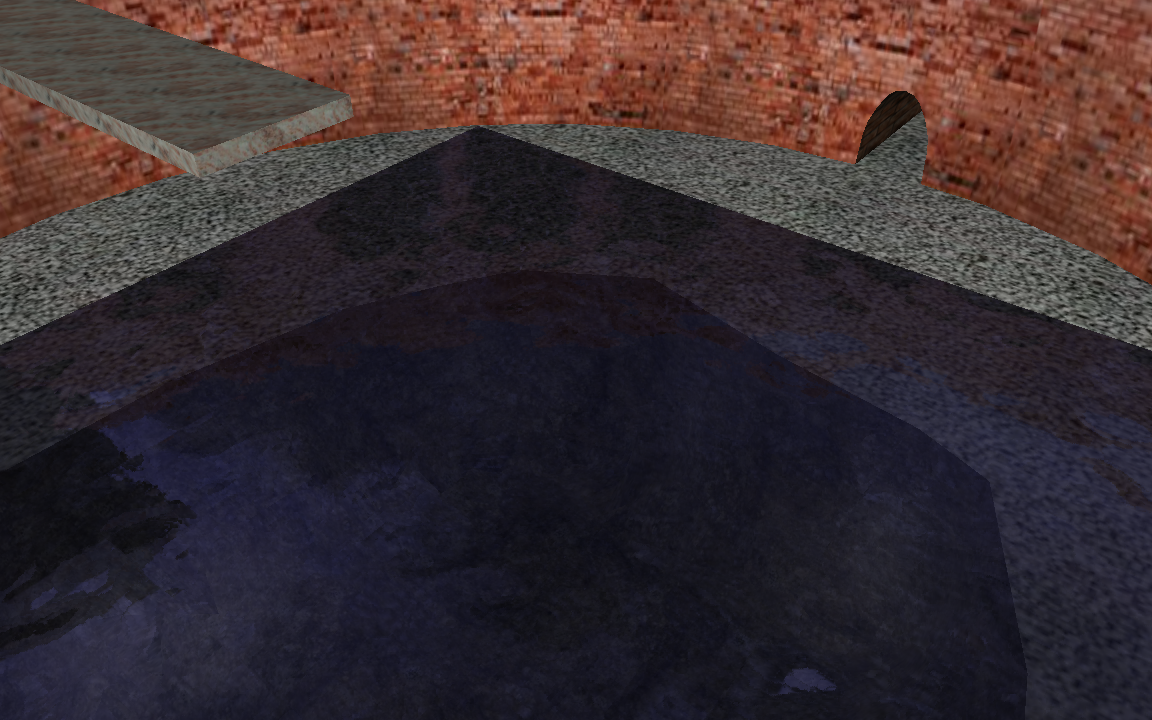
\includegraphics[width=2.0in]{water_shaders_3}
  \caption{Water using our effects: 1) Per-pixel lighting and bump mapping.
2) Per-pixel lighting and reflections and refractions (by a single environment cube map texture).
3) All effects.}
  \label{fig_water}
\end{figure*}
\setcounter{figure}{5}

\section{Defining custom plug points}

In your shader code, you can define new plug points by a
magic comment:

\begin{mycode}
\begin{Verbatim}[commandchars=\\\{\},fontsize=\small]
/* PLUG: name (param1, param2, ...) */
\end{Verbatim}
\end{mycode}

This defines a point where calls to user functions declared as
\texttt{PLUG\_name} will be inserted. They will be called with given
parameters.

Many effects may use the same \texttt{PLUG\_name},
you can even use the same \texttt{PLUG\_name} many times within a single
effect. All the \texttt{PLUG\_name} functions
will be uniquely renamed to not collide with each other.

The calls will be added in the order they are specified on the
\texttt{effects} list. More precisely, the most local effects
(at light sources and textures) are called first, then the effects
at shape appearance, and finally the effects inside the grouping nodes.
Although, preferably, for most effects this order will not matter.

A plug is often defined to allow modifying some parameter
repeatedly (like adding or modulating the fragment color),
so one or more of the parameters are often allowed to be handled
as \texttt{inout} values.

The same plug name may be declared many times in the source shader.
This means that a single \texttt{PLUG\_xxx} function will be called
many times. For example, this is useful when your shader calculation is naturally
expressed as a loop, but you had to unroll this loop for shader source
(for example, to slightly tweak some loop iterations).
The plug names that are available per-light source and per-texture
are an example of this.
%% If you use the \texttt{PLUG\_texture\_color}
%% inside \texttt{Appearance.effects}, you change the color of all
%% the textures (even shader textures).
%% Not really available, as params to texture\_color differ.
If you use the \texttt{PLUG\_light\_scale}
inside \texttt{Appearance.effects}, you change the intensity
of all the light sources on the given shape. Contrast this with using
the same \texttt{PLUG\_light\_scale} inside a \texttt{X3DLightNode.effects},
where you only change the given light node contribution.

Currently all the plugs must be procedures, that is their result type
must be declared as \texttt{void}. We have been considering
a possibility of functions, where part of the calculation may be replaced
by a call to a plugged function. While not difficult to implement,
this idea seems unnecessary after many tests.
Procedural plugs are easier to declare, as the call to the plug
may be simply inserted, while in case of function it will have to replace
some previous code. This also means that using a procedural plug
\textit{never} replaces or removes some existing code, which is a very nice
concept to keep. We want the effects to cooperate with each other,
not to ,,hijack'' from each other some parts of the functionality.

The nice feature of our magic \texttt{/* PLUG ... */} comments is that a shader source
is still valid even if you completely ignore the plugs. For example,
you can write a custom \texttt{ComposedShader} node, defining some plugs,
and for X3D browsers that understand them --- the plugs can be used,
for other browsers --- plugs will be gracefully ignored (but still
the shader will run, although without any effects).

You can define new plug points in your own effects code, as well as in your
complete custom shaders (like \texttt{ComposedShader}) code.
In the first case, the plug points
are only available for the following effects of the same node.

\subsection{Where the forward declarations are placed}

Special comment \texttt{/* PLUG-DECLARATIONS */} may be used
near the beginning of your shader source code. It is only useful
if your shader code defines any new plugging points, that is if you
have any magic \texttt{/* PLUG: ... */} comments inside.
When some other effect uses your plugging point, the renderer adds
an appropriate call to a function in that effect.
Additionally, the renderer has to declare the function,
because it may be in a separate compilation unit (in case of GLSL),
or just defined later in the code.
These (forward or external) declarations are inserted at
the point of special \texttt{/* PLUG-DECLARATIONS */}
comment, or (when it is missing) simply at the beginning of your shader source.
%% This applies in the same way to shader code inside an \texttt{EffectPart},
%% or inside standard X3D node like \texttt{ShaderPart}.

Using \texttt{/* PLUG-DECLARATIONS */} may be necessary
as some shading language directives are required to be placed before
all normal declarations. For example, in case of the \emph{OpenGL shading language},
the \texttt{\#version} as well as some \texttt{\#extension} directives
must occur at the beginning of the shader code. You should place
\texttt{/* PLUG-DECLARATIONS */} after such directives,
and before any \texttt{/* PLUG: ... */} declarations.

\subsection{Invalid shader code}

We guarantee the behavior only if the provided shading language code
is a correct, self-contained code. The errors (like unterminated block)
%%  (,,\texttt{\{}'' without matching ,,\texttt{\}}'')
%% ,
%% or an unterminated comment)
may only be detected after the complete shader
is determined and compiled by the GPU.
It should be noted that for shading languages with separate compilation units,
the parsing errors can be at least reported always for the correct code piece
(effect part).

The \textbf{application does not need to parse the shader code} at any point.
%% Still, by writing incorrect code,
%% you can cause the whole shader to malfunction.
%% is actually better, and

%% In all our practical tests, this approach didn't cause any problems.
%% Since you can implement each effect separately, you can also test them separately,
%% and in practice it's usually obvious where to look for the parsing error.

%% It should be noted however that in particularly nasty cases,
%% a deliberately poorly coded effect may cause troubles for other effects.
%% In particular, since you can use \texttt{\#define} and macros in your effect code,
%% you can do nasty tricks to break other effects. You can make them compile,
%% but function incorrectly. However, we don't consider
%% it a real problem. You really have to deliberately want to do something bad,
%% and be familiar with internals about how the shader is generated,
%% to achieve some particular weird behavior.
%% It doesn't happen by accident in our experience.
%% %% And you may need to use the internal knowledge
%% %% how the other effects are implemented (maybe how they are implemented
%% %% inside the browser).

%% Note that this isn't a security problem --- bad shader code only breaks
%% rendering of a particular shape. And X3D \texttt{ComposedShader} node allows users
%% to execute any shading language code anyway. So if there's anything dangerous
%% (for example a buggy OpenGL may cause the browser process to exit with
%% segmentation fault on some special shader code snippets),
%% you could do it without using our effects framework anyway.

\section{Examples}

Effects may define and use their own uniform variables, including textures,
just like the standard shader nodes. So we can combine any number of textures
inside an effect. As an example we wrote a simple effect that mixes a couple of
textures based on a terrain height (see figure \ref{fig_terrain}).
We could also pass any other uniform value to the effect, for example
passing the current time from an X3D \texttt{TimeSensor} allows to make
animated effects.

\begin{figure}[H]
  \centering
  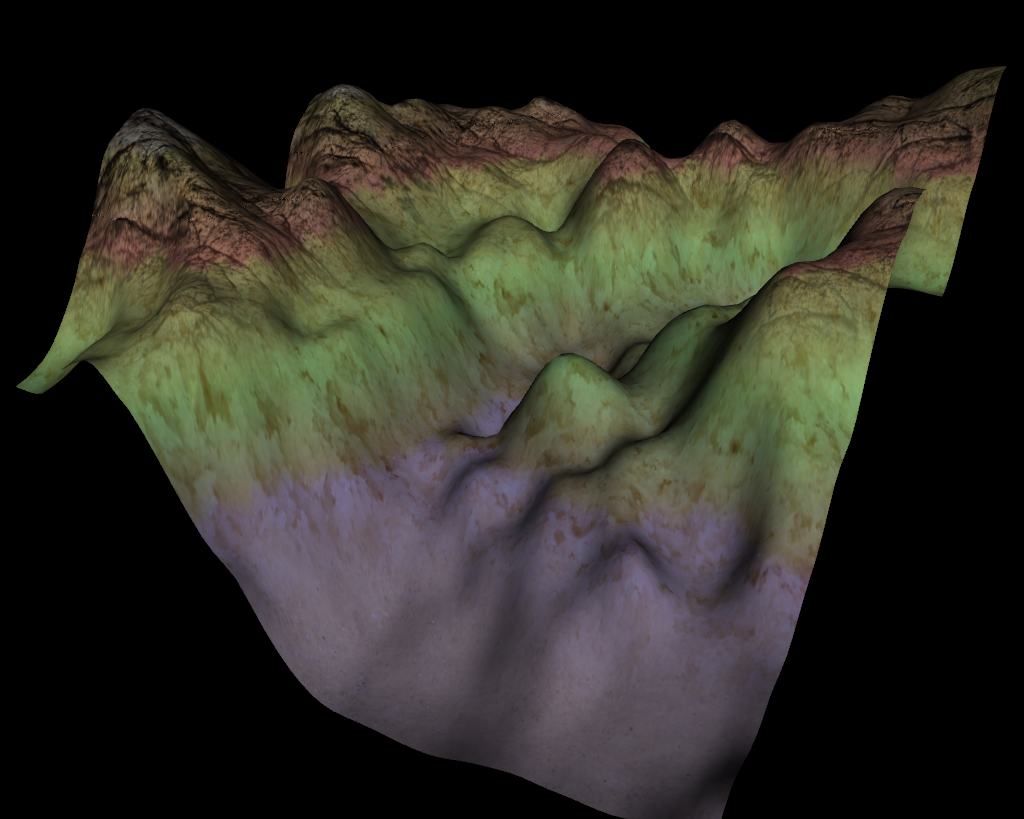
\includegraphics[width=2in]{terrain}
  \caption{ElevationGrid with 3 textures mixed inside the shader.}
  \label{fig_terrain}
%%based on the point height.}
\end{figure}

We can wrap 2D or 3D noise inside a \texttt{ShaderTexture}
(see figure \ref{fig_noise}).
A texture node like \texttt{NoiseTexture} from InstantReality
\cite{instant:noisetex}
may be implemented on GPU by a simple prototype using the \texttt{ShaderTexture}.

\begin{figure}[H]
  \centering
  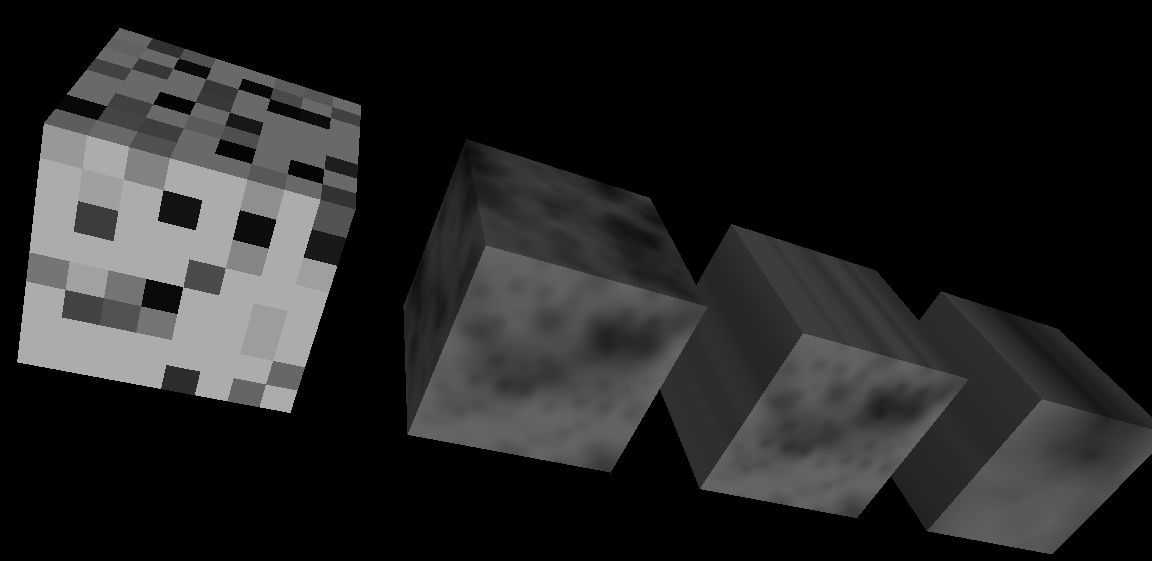
\includegraphics[width=2.2in]{noise-cropped}
  \caption{3D and 2D smooth noise on GPU, wrapped in a ShaderTexture.}
  \label{fig_noise}
\end{figure}

\emph{Water} is very nice to implement with the help of our effects,
as a proper water simulation
is naturally a combination of a couple effects.
To simulate waves we want to vary vertex
heights, or vary per-fragment normal vectors (for best results,
we want to do both things).
We also want to simulate the fact that water has reflections, and
is transparent. We have implemented a nice water using this approach,
with (initially) two independent effect nodes. See figure \ref{fig_water}.
Then we have tested two alternative
approaches for normal generation (take from pre-recorded series of normal-maps,
or calculate from a smooth 3D noise). They both generate normal
vectors in the tangent space, overriding a plug defined by yet another effect
that transforms normals into the eye space.
This way we have extracted all the common logic into a separate effect,
making it clear where the alternative normal generation methods differ
and what they have in common.

%% Our approach also allowed us to easily implement and test
%% two alternative versions for generating water normals.
%% One approach was to take normals from the pre-recorded sequence of images
%% (encoded inside \texttt{MovieTexture},
%% with noise images generated by the \emph{Blender} renderer).
%% The second approach was to calculate normals on the GPU from
%% a generated smooth 3D noise. Thanks to our effects system,
%% we could immediately test our alternative normal vector approaches,
%% without touching the water reflection / refraction effect.
%% Moreover, the implementations of these two approaches are concerned
%% only with calculating the normal vectors in the object space.
%% They override a special plug of yet another effect, that transforms
%% these normal vectors into the eye space.
%% This way we have extracted all the common logic into a separate effect,
%% making it clear where the alternative versions differ and what they have
%% in common.
%% This was possible because one effect can define
%% new plug names, that can be used by the other effects.

%% (As for the results about which one is better: predictably, we showed
%% that using GPU noise is slower, requires a better GPU,
%% but also improves the quality noticeably. With GPU noise, there is no problem
%% with aliasing of the noise texture, and the noise parameters can be adjusted
%% in real-time.)

We also have plugs to change the geometry in object space.
%% Again, since the effect is integrated with all the browser shaders,
%% you only need to code a simple function to change the vertex positions
%% as you want. The effect instantly works with all the lighting and texturing
%% conditions.
Since the transformation is done on GPU, there's practically
no speed penalty for animating thousands of flowers in our test scene.
See figure \ref{fig_flowers}.

\setcounter{figure}{8}
\begin{figure}[H]
  \centering
  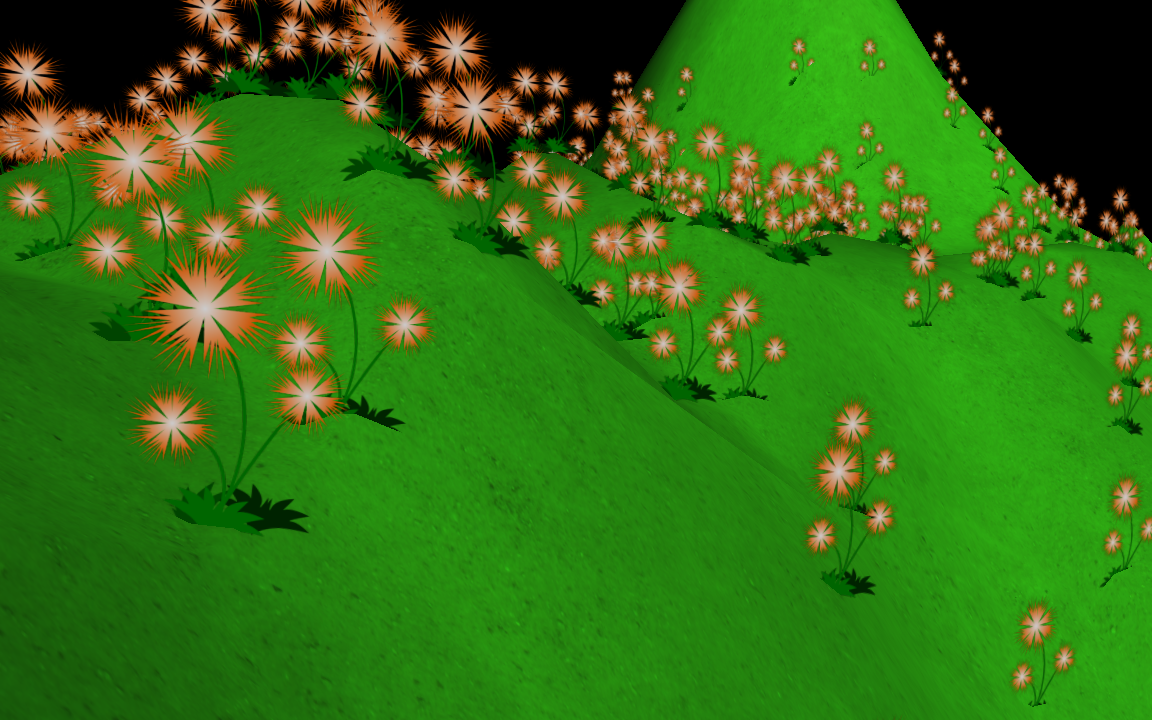
\includegraphics[width=2in]{flowers}
  \caption{Flowers bending under the wind, transformed on GPU in object space.}
  \label{fig_flowers}
\end{figure}

We would like to emphasize that all the effects demonstrated here
are theoretically already possible to implement using the standard
X3D \textit{Programmable shaders component} \cite{x3d:shaders}. However, such implementation
would be extremely cumbersome.
You would first have to implement all the necessary (multi-)texturing, lighting,
shadows, and other rendering features in a shader code.
This is a large work if we consider all the X3D rendering options, and note that
a shader should remain optimized for a particular setting.
%% Actually, it isn't even possible, unless we can calculate some global options,
%% like which light sources and fog nodes affect the given shape.
The only manageable way to do this, that would work for all the lighting
and texturing conditions, is to write a shader generator program.
Which is actually exactly what our effects already do for you ---
the implementation of our effects constructs and links
the appropriate shader code, gathering the information from all the nodes
that affect the given shape. And all the information is nicely integrated
with X3D nodes, effects are specified at suitable nodes, and their
uniform values and attributes are integrated with X3D fields.

Many complete example models using our effects
are available inside our engine demo models on
\URL{http://vrmlengine.sourceforge.net/demo_models.php}.
The relevant demos are mostly inside the \texttt{compositing\_shaders}
subdirectory, also the \texttt{water} subdirectory contains
the mentioned water effects.
You can open these examples using any of our engine tools,
like \texttt{view3dscene}.

%% You can run \texttt{view3dscene} with \texttt{--debug-log-shaders} command-line
%% option. Output will show you the final shader code generated,
%% and also the OpenGL log after linking the shaders.
%% %% Be sure to redirect the output to a file, and you may want to test it first
%% %% with a simple scene with one shape --- as the output may be quite large.
%% This is a useful way to learn about our shader rendering internals.

%% Another useful option to try in \texttt{view3dscene} is to switch to
%% \textit{View $\rightarrow$ Shaders $\rightarrow$ Enable For Everything} mode.
%% This will force shader rendering for all the shapes,
%% while by default we use shader rendering only for the shapes that
%% require particular effects (shaders by \texttt{ComposedShader}, effects
%% described in this paper, shadow maps and such).
%% Forcing shader rendering for everything allows to see
%% how our shaders implement the whole X3D lighting and texturing model.
%% It also forces all the lighting calculation to be done per-pixel, resulting
%% in perfect specular highlights and spot light shapes.

%% Development notes: only the SVN demo\_models contain
%% compositing\_shaders subdirectory.
%% You also have to use view3dscene from SVN or nightly builds,
%% see \URL{http://michalis.ii.uni.wroc.pl/vrmlengine-snapshots/}.

\section{Implementation notes}

We have implemented all the X3D extensions described in this paper
for the \emph{OpenGL Shading Language} (GLSL).
However, we have designed our extensions
to be applicable to other shading languages as well (like Cg or HLSL),
and we believe they can be handled in a similar fashion.
In particular, we have tested that the \emph{separate compilation units}
concept of GLSL, while very useful, is not necessary for proper implementation
of our effects.

%% concept, that is specific to GLSL, is useful here:
%% it forces
%% cleaner shader code (you cannot use undeclared functions from other
%% shader parts) and it gives you better line numbers in error messages
%% (although a pre-processor directive like \texttt{\#line} could also be used for
%% this).

%% and we think that the same set of plugs will be useful for them --- but it's just a theory.
%% An implementation of our effects for other shading languages may
%% find other opportunities for plugging points.
%% In particular, we have tested that the \emph{separate compilation units}
%% of GLSL are not necessary for a correct implementation of our effects.
%% We also believe that most of our plug points (like ,,do something in object space'',
%% ,,do something in eye space'') are generic enough to be usable
%% with all shading languages.

\section{Conclusion}

We show a new approach for developing effects using the GPU shading languages.
It allows to combine various shader effects with each other
and with application internal shaders.
Our approach is relatively easy
to implement, and allows the authors to directly use the existing GPU shading
languages.
We propose a number of extensions to the X3D,
an open standard for 3D data, to make our effects available for 3D
content authors. We have implemented our approach for the GLSL shading language.

%% \section*{Acknowledgements}

%% A lot of people helped and encouraged the development of our VRML/X3D engine,
%% with it's rendering features and extensions. A big ,,thank you''
%% goes to all of you.

\bibliographystyle{eg-alpha}
% \nocite{*}
\bibliography{compositing_shaders}

\end{document}
